
\chapter{视频动作捕捉动画生成}
动作捕捉(MoCap, Motion Capture)是指利用多种传感器,如光感、惯性、摄像头等,来记录物体或人体运动过程中的动作的技术。在军事、影视、运动、医疗、机器人、计算机视觉及图形学等领域有着广泛且深入的应用。本章针对动作捕捉在电影制作、游戏开发等需要将动作绑定至角色模型制作三维动画的场景,利用深度学习人体姿态估计,对RGB单目单人视频中的人体动作进行提取,再绑定至角色模型,搭建低门槛、低成本、广泛场景的视频动作捕捉解决方案。

\section{整体框架}

视频动作捕捉动画生成的整体流程如图x所示,首先利用RGB摄像头,如手机摄像头,采集单人运动视频。第一步将视频送入第三章中的二维人体姿态估计模型对每一帧中的主要人物目标的各关节坐标进行估计。第二步将得到的二维坐标序列送入第四章的三维人体姿态估计模型进行三维坐标的估计。第三步,搭建人体骨骼模型,将三维坐标序列转换为描述骨骼运动的欧拉角序列,并写为bvh动作描述文件。第四步创建人体角色模型,利用动画生成软件将bvh文件描述的动作序列绑定至模型。最终生成三维动画,可在动画引擎中进行播放。
\begin{figure}[h]
	\centering
	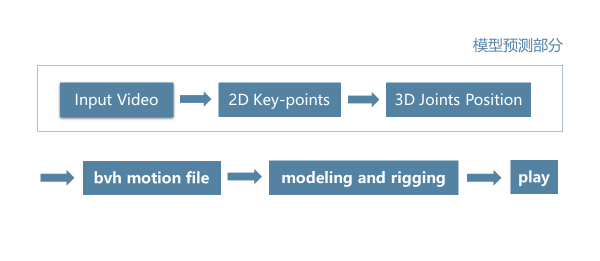
\includegraphics[scale=0.4]{figures/27.png}
	\caption{视频动作捕捉动画生成整体框架}
	\label{fig:f27}
\end{figure}

\section{实现细节}
\subsection{Bvh文件设计}{}
综合考虑人体姿态信息的多样性和复杂性,为了最大限度表达人体姿态,同时考虑数据量因素,现该领域研究人员一般用人体各个关键点来估人体姿态信息。基于骨骼关键点方法首次由  Johansson 在其经典的移动灯显示实验提出。人体姿态的大部分信息由主要的关节关键点即可描述。由此,人体姿态估计领域的研究大多基于该描述方法。目前主流的数据集的标签也采用标注骨骼关键点的方式。例如上述Human3.6m数据集中的人体骨骼关节点定义如图\ref{fig:f12}所示。在本文进行三维人体姿态估计时,以上人体骨骼模型也成为了由模型预测结果转为动作描述文件的基础。
由上一小节中对bvh文件的介绍可知,每个bvh文件描述一个运动目标,且运动目标由各个关节点构成,并以继承关系构建为骨骼树,具有唯一的父节点。故而对于本文所采集运动信息的人体目标,保留了21个人体关键关节点,设计并搭建了人体骨骼架构,具体的父子节点关系如下:

\begin{lstlisting}[language=python, label={lst:children}]
 self.children = {
    'Hip': ['RightHip', 'LeftHip', 'Spine'],
    'RightHip': ['RightKnee'],
    'RightKnee': ['RightAnkle'],
    'RightAnkle': ['RightAnkleEndSite'],
    'RightAnkleEndSite': [],
    'LeftHip': ['LeftKnee'],
    'LeftKnee': ['LeftAnkle'],
    'LeftAnkle': ['LeftAnkleEndSite'],
    'LeftAnkleEndSite': [],
    'Spine': ['Thorax'],
    'Thorax': ['Neck', 'LeftShoulder', 'RightShoulder'],
    'Neck': ['HeadEndSite'],
    'HeadEndSite': [],  # Head is an end site
    'LeftShoulder': ['LeftElbow'],
    'LeftElbow': ['LeftWrist'],
    'LeftWrist': ['LeftWristEndSite'],
    'LeftWristEndSite': [],
    'RightShoulder': ['RightElbow'],
    'RightElbow': ['RightWrist'],
    'RightWrist': ['RightWristEndSite'],
    'RightWristEndSite': []
}
\end{lstlisting}
进一步地,基于人体解剖学知识,将各个子关节相对于父关节的初始偏移方向定义如下:
\begin{lstlisting}[language=python, label={lst:direction}]
self.initial_directions = {
    'Hip': [0, 0, 0],
    'RightHip': [-1, 0, 0],
    'RightKnee': [0, 0, -1],
    'RightAnkle': [0, 0, -1],
    'RightAnkleEndSite': [0, -1, 0],
    'LeftHip': [1, 0, 0],
    'LeftKnee': [0, 0, -1],
    'LeftAnkle': [0, 0, -1],
    'LeftAnkleEndSite': [0, -1, 0],
    'Spine': [0, 0, 1],
    'Thorax': [0, 0, 1],
    'Neck': [0, 0, 1],
    'HeadEndSite': [0, 0, 1],
    'LeftShoulder': [1, 0, 0],
    'LeftElbow': [1, 0, 0],
    'LeftWrist': [1, 0, 0],
    'LeftWristEndSite': [1, 0, 0],
    'RightShoulder': [-1, 0, 0],
    'RightElbow': [-1, 0, 0],
    'RightWrist': [-1, 0, 0],
    'RightWristEndSite': [-1, 0, 0]
}
由此构成了人体骨骼模型的默认形态。
在人体解剖学中,骨骼的运动由关节运动主导,关节的运动与关节面形状贴合,而关节面形状也是在人体的长期活动中,肌肉作用下逐步获得、形成的,以上击力使得人体关节运动一般为绕某个轴进行的旋转运动。在上述简化的人体骨骼模型下,每个骨骼的旋转平面皆可由其他骨骼的方向定义,这为构造bvh文件数据部分的欧拉角任务提供了清晰明确、易于定义的旋转轴。故而针对根节点,即Hip节点保留3个Translation和3个Rotation共6个通道,其余子节点仅保留3个Ratation通道。生成的bvh文件样例附于附录。

\end{lstlisting}
\subsection{三维角色动作绑定}{}
在进行三维角色动画创作的过程中,当已经创建了一个骨骼结构的动作后,需要将动作与目标的实际模型进行捆绑,使得动作可以在目标模型上展示和播放,这个过程通常称为三维动画角色动作绑定或骨骼绑定(3D character rigging for animation)。
在本文的框架中,我们选择使用Autodesk的MotionBuilder软件,将上一小节生成的bvh文件与已有的人物模型进行绑定,MotionBuiler软件的图形工作界面如图\ref{fig:f28}所示。本文的工作利用其提供的Python借口进行动画的自动化生成。
\begin{figure}[h]
	\centering
	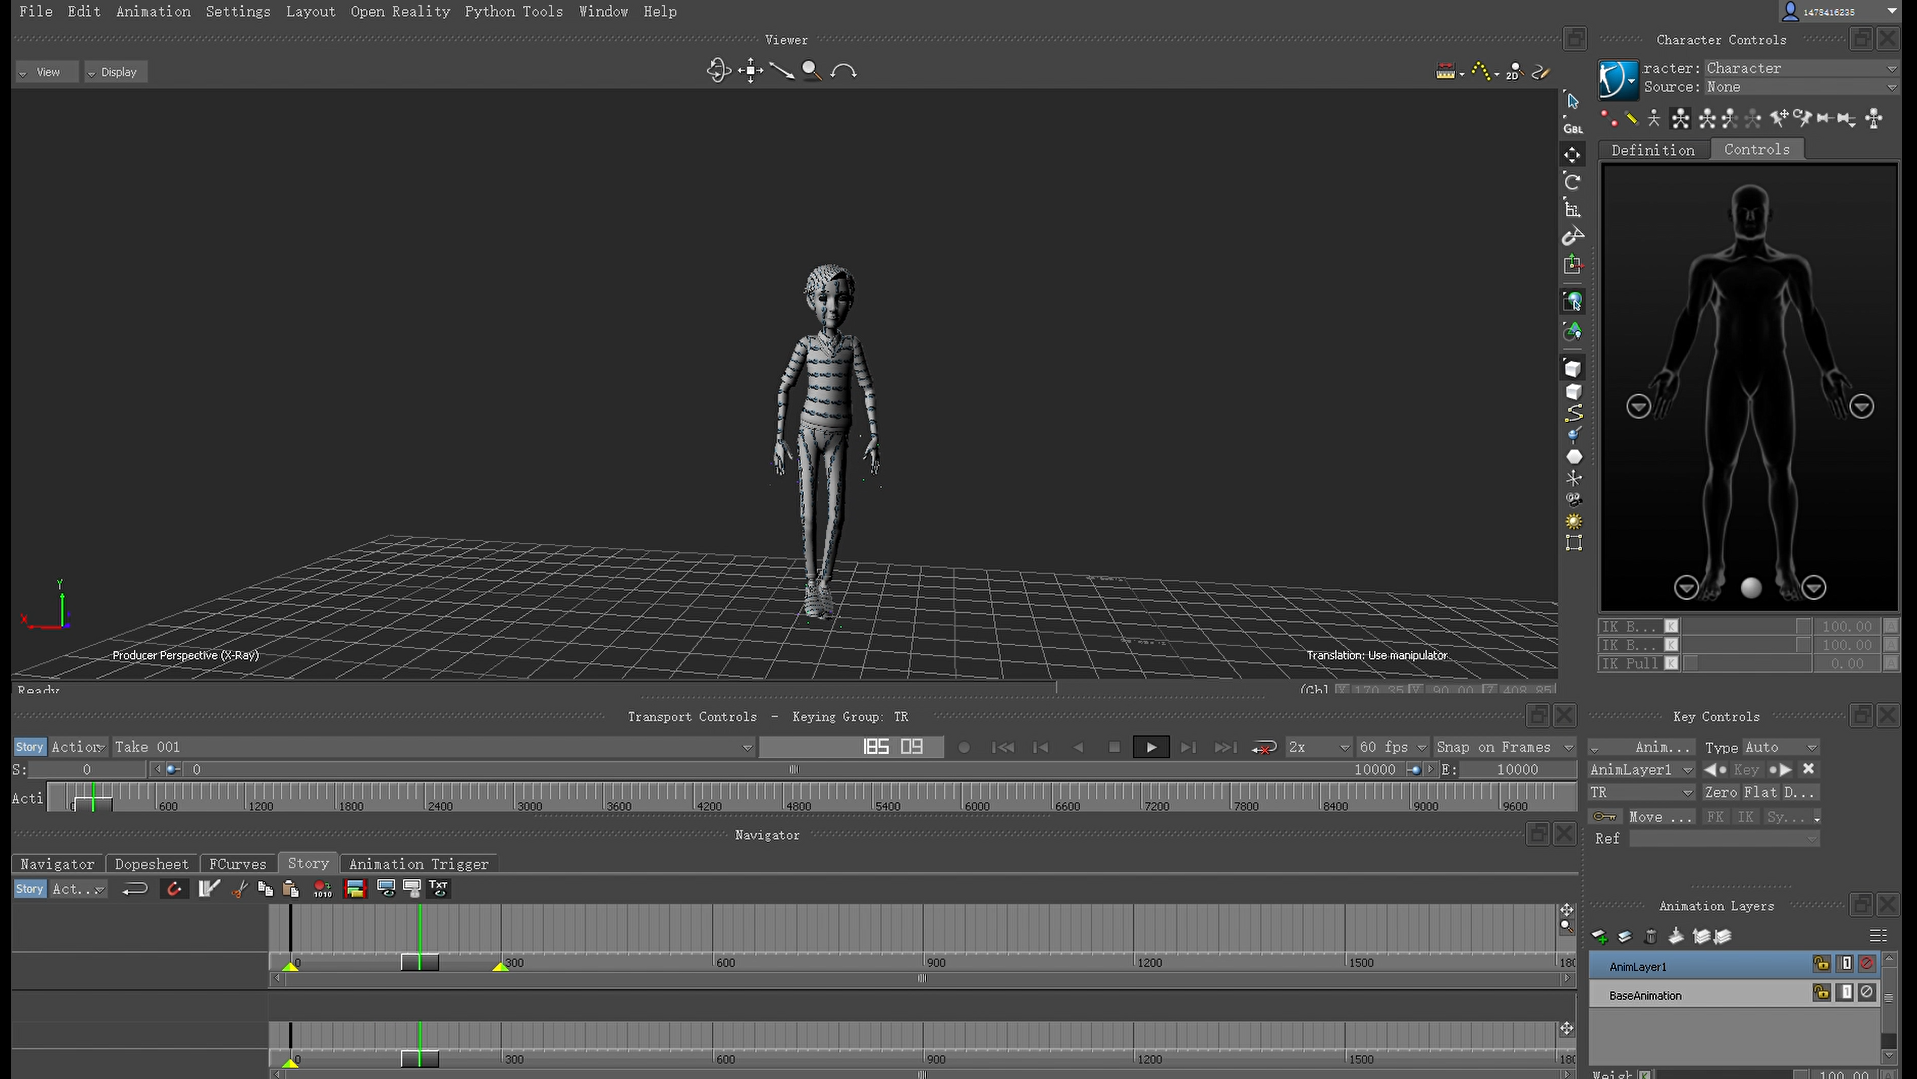
\includegraphics[scale=0.4]{figures/28.png}
	\caption{MotionBuilder图形工作界面}
	\label{fig:f28}
\end{figure}


\section{实现效果}
\subsection{人体姿态估计}{}
本文选取了网络视频,对其进行人体姿态估计结果如图\ref{fig:f29}所示。
\begin{figure}[h]
	\centering
	
\includegraphics[scale=0.4]{figures/XJTU_RED.png}
	\caption{自选视频的三维人体姿态估计结果}
	\label{fig:f29}
\end{figure}
在估计的过程中,三维姿态结果出现了偶然的不稳定情况,会出现突发的错误帧。在本文第四章中,指出了三维姿态结果对二维姿态结果的强依赖关系,本文针对此设计了对照实验,将我们的模型与将二维关节点真实坐标输入第四章模型输出的结果做了对比,如图\ref{fig:f30}所示。结果证明输出结果中出现的动作错乱的主要原因为二维关节点的识别和估计错误,可根据需要利用卡尔曼滤波进行平滑。
\begin{figure}[h]
	\centering
	\includegraphics[scale=0.4]{figures/30.png}
	\caption{输入为真实二维标注与二维估计模型预测结果的三维估计结果对比}
	\label{fig:f30}
\end{figure}

\subsection{动作绑定}{}
将上述模型对视频的预测结果,即三维关节点坐标转换为了关节旋转欧拉角,按照前述bvh文件设计生成了相应的bvh文件。在MotionBuilder软件中,对已有的人体角色模型进行了动作绑定,软件界面如图x,绑定结果如图x。